\documentclass{article}
\usepackage[utf8]{inputenc}
\usepackage{latexsym, amssymb, amsmath, amsfonts, amscd, amsthm, xcolor, pgfplots}
\usepackage[margin=1in]{geometry}
\usepackage{verbatim}
\usepackage{float}
\usepackage{cite}
\usepackage{lipsum}
\usepackage{hyperref}\hypersetup{
    colorlinks=true,
    linkcolor=blue,
    filecolor=magenta,      
    urlcolor=cyan,
}
\usepackage{cleveref}

\title{CS598: Deep Generative \& Dyn. Models\\
       Project Proposal: Learning Structured Mappings for Finite Element Problems}
\author{Nicolas Nytko, Sean Farhat, Nathanael Assefa, (Alexey Voronin)}
\date{\today}

\begin{document}

\maketitle

\section{Introduction}

Partial Differential Equations (PDEs) provide a mathematical framework for describing and understanding many physical phenomena in science and engineering, from the behavior of fluids and materials to the dynamics of electric and magnetic fields. The solution of PDEs is essential for making predictions, designing and optimizing systems, and developing new technologies. Solving PDEs analytically can be challenging, and in many cases, it is impossible. Therefore, numerical methods are often used to approximate the solutions of PDEs.

To solve numerical PDEs, one must turn the continuous problem into something discrete that is solvable on a computer: this is commonly done by the finite element method (FEM), where a problem domain is approximated by a discrete triangulation (mesh) upon which the PDE is satisfied discretely (think Taylor approximation). Once the PDE has been discretized and approximated, the resulting system of equations is solved numerically such that the solution minimizes the residual on the mesh.  What algorithm we use to solve the system, and thus how fast we can solve it, depends on various properties of the mesh and the problem itself.

We want to learn how to map PDE discretizations from unstructured (irregular) mesh domains to structured (grid-like) ones, just like in~\Cref{fig:meshes}. To make this happen, we will treat it as a generative process where we wish to generate data from a source distribution: the structured operators. This can be achieved via a diffusion process where we take the structured operator, iteratively add ``noise'', and then learn the ``de-noising'' process.  Our noise is not the simple Gaussian noise applied to images; instead, we will perturb each of the coordinates and re-triangulate (via an out-of-the-box triangulation algorithm such as Delaunay) to obtain a new discretization. Additionally, we will add a regularization term to keep the solution of the new ``noised'' operator close to the solution of the original structured one. We will ideally have a network that will take in any unstructured operator (analogous to a fully noised operator), and it will ``de-noise'' the linear system until it reaches a structured operator that realizes the same solution.


\begin{figure}[!ht]
      \centering
      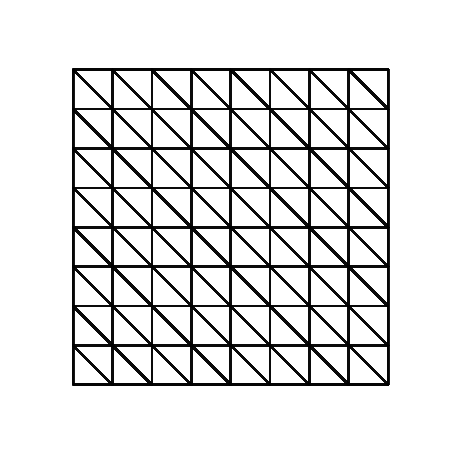
\includegraphics[width=.35\textwidth]{./figures/meshes/structured.pdf}
      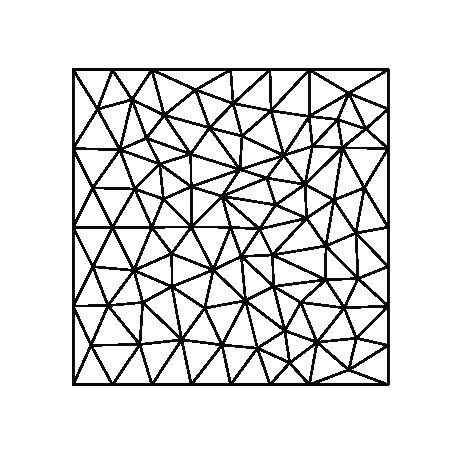
\includegraphics[width=.35\textwidth]{./figures/meshes/unstructured.pdf}
      \caption{Example of triangular meshes: structured (left) and unstructured (right). } \label{fig:meshes}
\end{figure}

%
\section{Motivation}
Multigrid methods~\cite{RugeAMG1987,BriggsMgridTut} are a family of fast iterative solvers for sparse linear systems, such as ones that arise from the numerical discretization of PDEs using the finite element method~\cite{ClaesFEM}.  Much of the speedup in using multigrid solvers is obtained by constructing a hierarchy of smaller, easier-to-solve problems, then interpolating approximate solutions between different levels.  There has been a wealth of theory dedicated to creating such a problem hierarchy on regular, well-structured problem domains; however, for more complex problem domains, we often must switch to using algebraic methods, which are often based on heuristics and can vary in efficacy. 

We propose to learn a mapping from unstructured problems to structured ones in order to create a more efficient multigrid solver. By transferring solutions to and from a related structured problem, we can reuse existing black-box geometric multigrid algorithms that will converge very well for the overall problem. 
%
\section{Data}
We will generate structured problems using triangular finite-element discretizations of the diffusion equation,
\begin{equation}
\nabla \cdot (\kappa(x,y)\nabla u) = 0, \label{eqn:diffusion}
\end{equation}
where $\kappa(x,y)$ is the diffusivity of the material at some point and $u(x,y)$ is the unknown density we would like to solve for.  To add variance in the set of problems we want to \textit{diffuse from}, we will randomly generate $\kappa(x,y)$; for example, by using simplex noise~\cite{simplex} or polynomial interpolation to obtain the function values.  To generate the actual matrices themselves, we will use the Firedrake library~\cite{Firedrake,FRathgeber_etal_2017a} on \cref{eqn:diffusion}, giving us a set of linear systems
\begin{equation}
A^{(i)} u^{(i)} = b^{(i)}.
\end{equation}
%
\section{Plan of Work}

\begin{itemize}
    \item Methodology for generating the dataset:
    \begin{itemize}
        \item Use triangular finite-element discretizations of the diffusion equation to generate structured problems.
        \item Randomly generate diffusivity values to add variance to the set of problems.
        \item Use Firedrake library to generate linear systems from the diffusion equation.
    \end{itemize}
    \item Learning approach for mapping unstructured problems to structured ones
    \begin{itemize}
        \item Use a generative process that involves iteratively adding noise to the structured operator and learning the de-noising process.
        \item Perturb each coordinate and re-triangulate to obtain a new discretization.
    \end{itemize}
    \item Loss function:
    \begin{itemize}
        \item Design a loss function that measures the difference between the predicted structured operator and the actual structured operator.
        \item Regularize the loss function to ensure the predicted operator is close to the actual solution.
    \end{itemize}
    \item Training the model:
    \begin{itemize}
        \item Train the model on the generated dataset of unstructured operators and corresponding structured operators.
        \item Validate the model on a separate test dataset.
    \end{itemize}
    \item Expected outcome:
    \begin{itemize}
        \item A deep neural network that can map unstructured PDE discretizations to structured ones.
        \item Improved efficiency of multigrid solvers for PDEs, particularly for complex problem domains.
    \end{itemize}
\end{itemize}
%
\section{Related Works}
\url{https://arxiv.org/abs/1104.0261}?
%
\bibliography{bibliography}
\bibliographystyle{plain}
\end{document}
